\documentclass[10pt,a5paper,twoside]{book}
\usepackage[tmargin=2.5cm,bmargin=2.5cm,lmargin=2.5cm,rmargin=2.0cm]{geometry}
\usepackage{fontspec}
    \setsansfont{Calibri}
    \setmainfont{Times New Roman}
\usepackage{tocbibind}
\usepackage{minted}
\usepackage{multirow}
\usepackage{graphicx}
\usepackage{blindtext}
\usepackage{tabularx}
\usepackage{eso-pic}
\usepackage{ragged2e}
\usepackage{xesearch}
    \SearchList*{itwords}{\emph{#1}}{%
        download,
        upload,
    }
\usepackage{setspace}
    \singlespacing
\usepackage{fancyhdr}
    \fancyhf{}
    \renewcommand{\headrulewidth}{0pt}
    \lhead{}
    \rhead{\thepage}
    \pagestyle{fancy}
\usepackage{titlesec}
    \titleformat{\chapter}[display]{\filcenter\fontsize{12}{12}\bfseries}{\chaptername \ \thechapter}{12pt}{\filcenter\fontsize{12}{12}\bfseries}
    \titlespacing*{\chapter}{0pt}{-50pt}{40pt}
    \titleformat*{\section}{\fontsize{12}{14}\bfseries}
    \titleformat*{\subsection}{\fontsize{12}{14}\bfseries}
    \titleformat*{\subsubsection}{\fontsize{12}{14}\bfseries}



\renewcommand{\bibname}{Daftar Referensi}
\renewcommand{\contentsname}{Daftar Isi}
\renewcommand{\listtablename}{Daftar Tabel}
\renewcommand{\listfigurename}{Daftar Gambar}
\renewcommand{\chaptername}{BAB}
\renewcommand{\figurename}{Gambar}
\newcommand{\var}[2]{\newcommand{#1}{#2}}
\newcommand{\pic}{Gambar}
\newcommand{\tab}{Tabel}
\newcommand{\code}{Kode}
%
% Hyphenation untuk Indonesia 
%
% @author  Andreas Febrian
% @version 1.00
% 
% Tambahkan cara pemenggalan kata-kata yang salah dipenggal secara otomatis 
% oleh LaTeX. Jika kata tersebut dapat dipenggal dengan benar, maka tidak 
% perlu ditambahkan dalam berkas ini. Tanda pemenggalan kata menggunakan 
% tanda '-'; contoh:
% menarik
%   --> pemenggalan: me-na-rik
%

\hyphenation{
    % alphabhet A
    a-na-li-sa a-tur 
    a-pli-ka-si 
    % alphabhet B
    ba-ngun-an 
    be-be-ra-pa 
    ber-ge-rak
    ber-ke-lan-jut-an 
    ber-pe-nga-ruh 
    % alphabhet C
    ca-ri
    % alphabhet D
    di-sim-pan di-pim-pin de-ngan da-e-rah di-ba-ngun da-pat di-nya-ta-kan 
    di-sim-bol-kan di-pi-lih di-li-hat de-fi-ni-si
    % alphabhet E
    e-ner-gi eks-klu-sif
    % alphabhet F
    fa-si-li-tas
    % alphabhet G
    ga-bung-an ge-rak
    % alphabhet H
    ha-lang-an
    % alphabhet I
    % alphabhet J
    % alphabhet K
    ke-hi-lang-an
    ku-ning 
    kua-li-tas ka-me-ra ke-mung-kin-an ke-se-pa-ham-an
    % alphabhet L
    ling-kung-an
    % alphabhet M
    me-neng-ah
    meng-a-tas-i me-mung-kin-kan me-nge-na-i me-ngi-rim-kan 
    meng-u-bah meng-a-dap-ta-si me-nya-ta-kan mo-di-fi-ka-si
    meng-a-tur
    % alphabhet N
    nya-ta non-eks-klu-sif
    % alphabhet O
    % alphabhet P
	pe-nye-rap-an 
	pe-ngon-trol
    pe-mo-del-an
    pe-ran  pe-ran-an-nya
    pem-ba-ngun-an pre-si-den pe-me-rin-tah prio-ri-tas peng-am-bil-an 
    peng-ga-bung-an pe-nga-was-an pe-ngem-bang-an 
    pe-nga-ruh pa-ra-lel-is-me per-hi-tung-an per-ma-sa-lah-an 
    pen-ca-ri-an peng-struk-tur-an
    % alphabhet Q
    % alphabhet R
    ran-cang-an
    % alphabhet S
    si-mu-la-si sa-ngat
    % alphabhet T
    te-ngah
    ter-da-pat
    % alphabhet U
    % alphabhet V
    % alphabhet W
    % alphabhet X
    % alphabhet Y
    % alphabhet Z
    % special
}
\var{\judul}{Rancang Bangun Layanan Platform as a Service (PAAS) untuk Mendukung Sistem Multi-Tenancy Pengembangan Aplikasi Berbasis Komputasi Awan}
\var{\penulis}{Putu Wiramaswara Widya}
\var{\nrp}{5111100012}
\var{\jurusan}{Teknik Informatika}
\var{\fakultas}{Teknologi Informasi}
\var{\prodi}{S-1}
\var{\bidangStudi}{Arsitektur dan Jaringan Komputer}
\var{\pembimbingSatu}{Royyana Muslim Ijtihadie, S.Kom, M.Kom, Ph.D.}
\var{\nipPembimbingSatu}{197708242006041001}
\var{\pembimbingDua}{Baskoro Adi Pratomo, S.Kom, M.Kom}
\var{\nipPembimbingDua}{510000003}



\makeatletter
\def\emptypage@emptypage{%
     \begin{center}
     Halaman ini sengaja dikosongkan
     \end{center}
     \newpage%    
}%
\def\cleardoublepage{%
        \clearpage%
        \if@twoside%
            \ifodd\c@page%
                % do nothing
            \else%
                \emptypage@emptypage%
            \fi%
        \fi%
}%
\makeatother

\begin{document}
    \title {\judul}
    \author {\penulis}


    \frontmatter
        \newpage
    \newgeometry{top=7cm}
    \large
    \sffamily
    \thispagestyle{empty}
    \color{white}
    \flushleft
    TUGAS AKHIR - KI091391 \\
    {\rmfamily\textbf{\MakeUppercase{\judul}}} \\*[32pt]
    \penulis \\*
    NRP \nrp \\*[10pt]
    Dosen Pembimbing 1 \\*
    \pembimbingSatu \\*[10pt]
    Dosen Pembimbing 2 \\*
    \pembimbingDua \\*[10pt]
    JURUSAN \MakeUppercase{\jurusan} \\*
    Fakultas \fakultas \\*
    Institut Teknologi Sepuluh Nopember \\*
    Surabaya, 2014 \\*
    \AddToShipoutPictureBG*{
\includegraphics[width=\paperwidth,height=\paperheight]{sampul.png}}
    \rmfamily
    \normalsize
    \restoregeometry
    \color{black}
    \cleardoublepage


        \newpage
    \centering
        \textbf{\MakeUppercase{\judul}} \\*[10pt]
        \textbf{\large{TUGAS AKHIR}} \\*
        Diajukan Guna Memenuhi Salah Satu Syarat \\*
        Memperoleh Gelar Sarjana Komputer \\*
        pada \\*
        Bidang Studi \bidangStudi \\*
        Program Stdui \prodi Jurusan \jurusan \\*
        Fakultas \fakultas \\*
        Institut Teknologi Sepuluh Nopember \\*[10pt]
        Oleh : \\*
        \textbf{\penulis} \\*
        NRP: \nrp \\

    \justify
        Disetujui oleh Dosen Pembimbing Tugas Akhir :\\*[20pt]
        \pembimbingSatu \hfil \hfill ............................ \\*
        NIP: \nipPembimbingSatu \hfill \hfill \centering (Pembimbing 1) \justify
        \pembimbingDua  \hfill \hfill ........................... \\*
        NIP: \nipPembimbingDua \hfill \hfill \centering (Pembimbing 2) \justify
    \cleardoublepage
 
        \chapter{Abstrak}
    \Blindtext[1][1]
    \cleardoublepage

        \chapter{Kata Pengantar}
    \Blindtext[1][1]
    \cleardoublepage

        \tableofcontents
            \cleardoublepage
        \listoftables
            \cleardoublepage
        \listoffigures
            \cleardoublepage



    \mainmatter
        \chapter{Pendahuluan}
    \section{Latar Belakang}
        \Blindtext[5][1]
    \section{Rumusan Masalah}
        \begin{itemize}
            \item \Blindtext[1][1]
            \item \Blindtext[1][1]
            \item \Blindtext[1][1]
        \end{itemize}
    \section{Batasan Masalah}
    \section{Tujuan}
    \section{Manfaat}
    \section{Metodologi}
    \section{Sistematika Laporan}
    \cleardoublepage

        \chapter{Landasan Teori}
    \section{Sebuah Tabel}
        \Blindtext[1][1]
        \begin{table}[h]
            \centering
            \caption{Contoh Tabel}
            \begin{tabular}{|l|l|l|}
                \hline
                Wiramaswara & Lalalala & Widya  \\ \hline
                Lelelele    & Lalalala & Lalala \\ \hline
            \end{tabular}
        \end{table}
        \Blindtext[1][1]
    \section{Sebuah Gambar}
        \Blindtext[1][1]
        \begin{figure}[h]
            \centering
            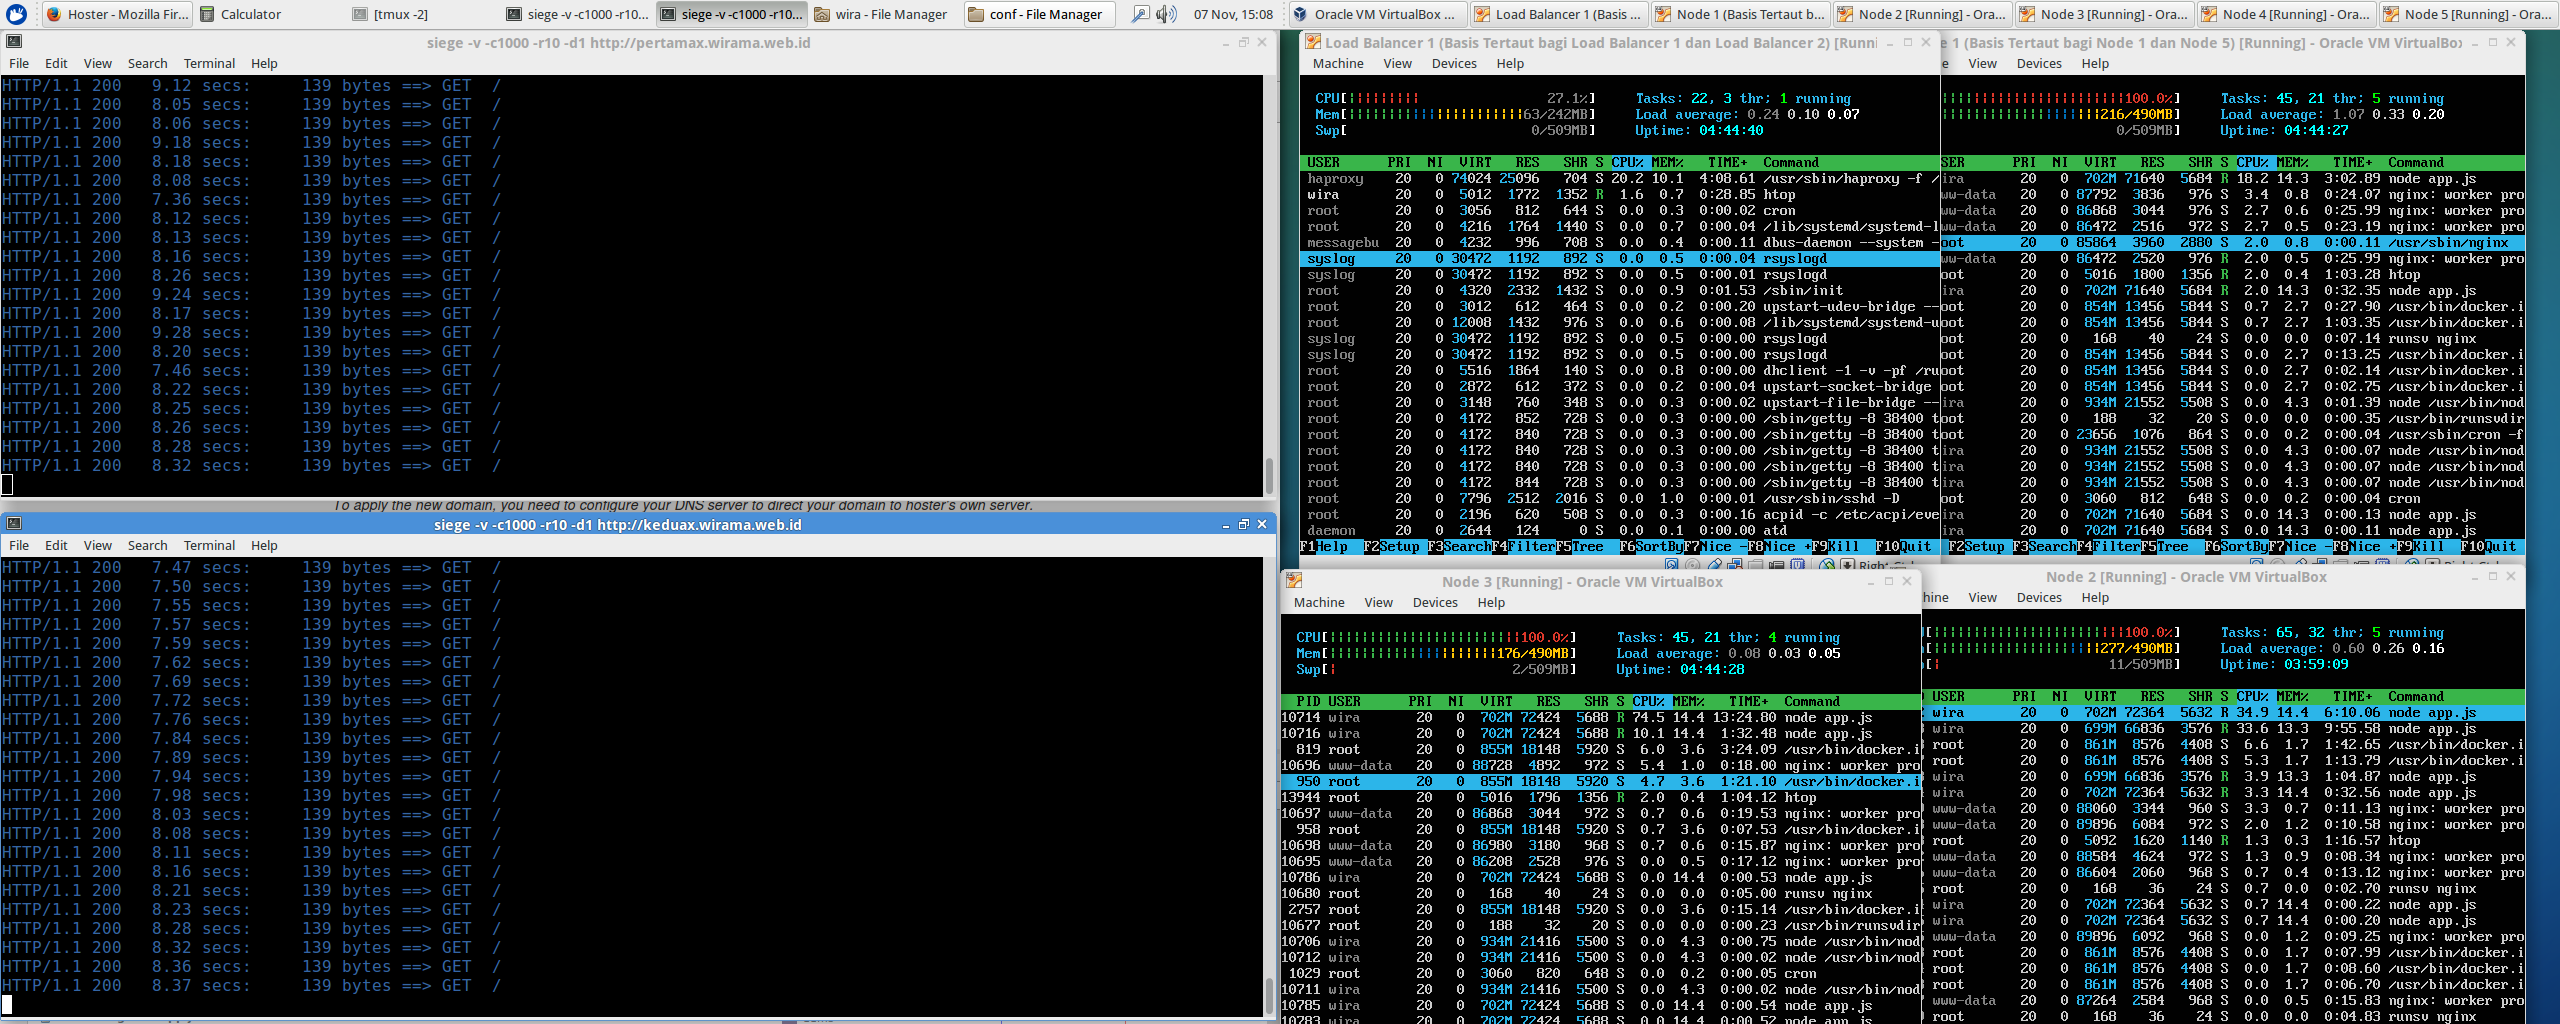
\includegraphics[width=1\textwidth]{tes.png}
            \caption{Coba gambar}
            \label{fig:testGambar}
        \end{figure}
    \section{Sebuah Kode}
        \begin{figure}[h]
            \begin{minted}{csharp}
string title = "This is a Unicode π in the sky"
const double pi = 3.1415926535
            \end{minted}
            \caption{Sebuah kode}
        \end{figure}
    \cleardoublepage

        \chapter{Analisis dan Desain}
    \section{Arsitektur Sistem}
        \Blindtext[5][1]
    \section{Kasus Penggunaan}
        \Blindtext[5][1]
    \section{Deskripsi Fitur}
        \Blindtext[5][1]
    \section{Rancangan Antarmuka}
        \Blindtext[5][1]
    \cleardoublepage

        \chapter{Implementasi}
    \section{Lingkungan Implementasi}
        \Blindtext[5][1]
    \section{Kode Program}
        \Blindtext[5][1]
    \section{Implementasi Antarmuka}
        \Blindtext[5][1]
    \cleardoublepage

        \chapter{Uji coba dan implementasi}
    \section{Lingkungan Uji Coba}
        \Blindtext[5][1]
    \section{Skenario Uji Coba}
        \Blindtext[5][1]
    \section{Uji coba performa sistem}
        \Blindtext[5][1]
    \cleardoublepage

        \chapter{Penutup}
    \section{Kesimpulan}
        \Blindtext[5][1]
    \section{Saran}
        \Blindtext[5][1]
    \cleardoublepage

\end{document}
